% This example An LaTeX document showing how to use the l3proj class to
% write your report. Use pdflatex and bibtex to process the file, creating 
% a PDF file as output (there is no need to use dvips when using pdflatex).

% Modified 

\documentclass{l3proj}
\begin{document}
\title{Team V - How Not To Kill Your Dog}
\author{Ross Adam \\
        Andrew Gardner \\
        Nicole Kearns \\
        Mamas Nicolaou \\
        Asset Sarsengaliyev}
\date{18 March 2013}
\maketitle

\chapter{Design}
\label{design}

This chapter covers the various aspects of the application's design process. As our project was client-based the design was very much focused on satisfying the requirements laid out in the previous chapter. Fiona Dowell, our client from Glasgow University's Veterinary School, evaluated our initial user interface design and we then revised it according to the feedback that we received from her. When we were satisfied with the design we moved on to the implementation phase.

\newpage

\section{Design Goals and Considerations}

The overall design goals for the application follow principles already well established in the field of web development.

These were:

\begin{enumerate} 
\item{\textbf{Precedence}} \\
The use of positioning, colour, size and contrast to naturally guide the user around the application. For example, most sites have a logo featured in the top left corner because studies have shown this to be the first place users look when accessing web sites. This enables natural navigation sequences: elements like the navigation bar being strategically placed so users' eyes will follow from the larger, relatively contrasted logo to the navigation bar.

\item{\textbf{Navigation}} \\
The principle of making it easy and intuitive for users to navigate your web site. For example, links and buttons should be well positioned and clearly indicate their function while offering appropriate feedback when clicked. Measures should also be taken to inform the user where they are currently within the application.

\item{\textbf{Typography}} \\
The text of a web application is the most common element of design and therefore deserves significant consideration. Font type, size, spacing and colour are essential to the application's overall clarity and readability.

\item{\textbf{Usability}} \\
The encompassment of previously defined principles such as precedence, navigability and text. They relate to how usable the application is for its users. An important usability consideration is that of 'standards adherence'. This is the following of conventions laid out and used by millions of other websites, such as underlined text indicating a link.

\item{\textbf{Consistency}} \\
The principle of making the application's design elements ``match'' coherently between pages and on the same page of the site. Attributes like colour and font choice, for example, should remain consistent across the site.

\item{\textbf{Clarity}} \\
The appropriate use of design techniques such as positioning, contrast, font aliasing and others to make your design stand out crisply and clear. 
\end{enumerate}
	
\subsection{Admin}

The admin user is solely responsible for the content management of the application. With that in mind we approached the admin interface's design with a heavy focus on usability and navigation, rather than fancy themes and textual styles. We felt that the admin interface should possess a natural gravitas; that it should be taken seriously as a tool that controls the entire functionality of the application and not as a novel feature. To this extent our goal was to use a very simple theme, contrasting sharply in style and presentation with the student user interface. This was a wilful breaking of the consistency design principle to enforce a measure of aforementioned seriousness onto the admin interface.

We also had to consider that the likely admins of the application would be relatively inexperienced with regards to administrating an entire web application's content. Being mindful of this we had to design the interface to be accommodating for the inexperienced, allowing for easy navigation and informative feedback with every action taken.

\subsection{Student}

In stark contrast to that of the admin user interface, the student's view of the web application had to embody all design goals previously defined in this chapter. They had to be able to navigate the site easily, knowing where they were at all times and how to get to where they would like to go with no fuss or ambiguity.

As this application's core functionality is assessment based it was important to have a gentle colour theme that would contrast naturally with the displayed content and not distract the user. This also held true with appropriate user feedback. We made an early design decision to provide the user with timely responsive feedback when answering questions.

An important design goal was to create an interactive learning experience for the user. In order to achieve this we decided to include an animal avatar with an associated health bar. A correct answer would have no effect whereas an incorrect answer would result in health loss. This design feature helps to engage the student on a personal level as their progress will affect the animal's lifespan. 

\section{Initial Design}

\subsection{ER Diagram}
	
After establishing our initial design goals we created an entity relationship diagram. Defining our data models at this phase allowed us to clearly understand the distinction between entities and how they relate to each other.


\subsection{Paper Prototypes}

Paper prototyping was an effective and inexpensive method used to determine the design direction of the student user interface. The use of paper prototypes allowed us to experiment with various design configurations without the overhead of time and resources. This method of design was particularly suited to this application as it was simple to review and to iterate upon. Client involvement was a requirement for the success of the project. Therefore it was imperative that our early design ideas were subject to client review and feedback. Sending several prototypes for client evaluation meant that there was more potential for varied, constructive feedback. Receiving said feedback from the client afforded us more opportunity to revise our designs in accordance with their wishes. 

The paper prototypes aimed to fulfil the student user's functional requirements as laid out in the previous chapter. This meant that we had to design mechanisms for the following use cases:

\begin{itemize}
\item{Viewing Topics\textbf{ (SR1)}}
\item{Viewing Slides\textbf{ (SR2)}}
\item{Viewing Questions\textbf{ (SR3)}}
\item{Answering Questions\textbf{ (SR4)}}
\end{itemize}

As will be discussed in the Prototype Evaluation section, our client indicated that two prototypes were particularly suitable in meeting the requirements of the application.

\begin{figure}[!htb]
\caption{Topic View}
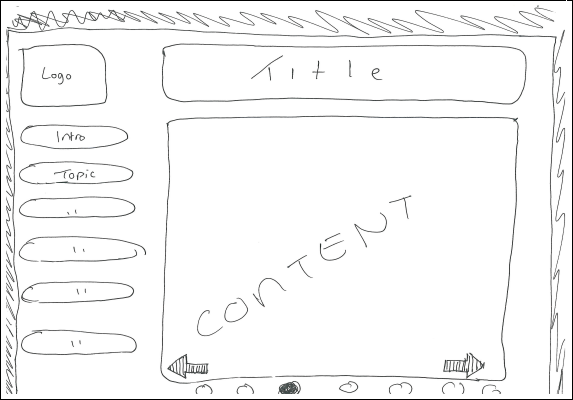
\includegraphics[width=\linewidth]{/users/level3/1002336a/TP3/team-project/Dissertation/images/Prototype2.png}
\end{figure}

\begin{figure}[!htb]  
\caption{Final Assessment}
 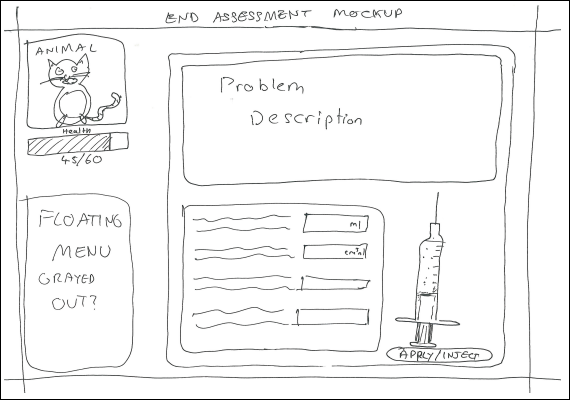
\includegraphics[width=\linewidth]{/users/level3/1002336a/TP3/team-project/Dissertation/images/Prototype1.png}
\end{figure}

The above-left image (\textbf{Fig 1.1}) shows the individual topic view for the student user interface. The ``title'' at the top of the page represents the topic's name, with the slides for the topic being shown in the ``content'' section. The arrows contained within the content section represents the possibility of a slider being used, enabling the user to easily switch back and forth between slides. The breadcrumbs, shown below the content box, were designed to enhance user navigability by allowing the user to directly select a slide to navigate to. The rounded buttons to the right of the content section represent clickable links to navigate between individual topics. These design elements satisfy requirements \textbf{SR1} and \textbf{SR2}.

This prototype satisfies design goals laid out in the beginning of this chapter. The judicious use of whitespace enhances the user interface's clarity. With regards to design precedence, the size of the content box (compared to other design features) functions as a focal point, demanding the user's attention. 

The above-right image (\textbf{Fig 1.2}) shows the final assessment page for the student user interface. The inclusion of an animal avatar and health bar satisfies the design goal of interactive student engagement, resulting in a heightened learning experience. Similar to \textbf{Figure 1.1}, the use of whitespace and size precedence allows the user to understand and easily navigate the interface presented to them. The problem description section represents the functional requirement \textbf{SR3} and the box below plus the apply/inject button represents the functional requirement \textbf{SR4}.  

We chose not to create a paper prototype of the admin interface because we knew that Django (the web framework we had chosen to implement the application with) would provide a suitable pre-defined interface. This will be discussed further in the Admin User Interface Subsection. 
 
\subsection{Prototype Evaluation}

The evaluation process involved sending the paper prototypes to our client, Fiona Dowell. This was an important part of the design process as her feedback would naturally impact the application's final design. 

With regards to the paper prototypes, the feedback confirmed our initial design choices. Both designs preferred by our team were also chosen by Fiona and her colleagues. The decision to revise and continue with these designs was reinforced by our client's feedback. This not only resulted in an easy design decision but also supported the overall design direction we had previously agreed on. While we knew further iteration and changes were likely required for implementation, we felt this was a solid base to start from.

\section{Interface Design}

This section covers the user interfaces for both admins and students, analysing how the design meets specific functional requirements and overall design goals.

\subsection{Admin User Interface}

\begin{figure}[!htb]
\caption{Admin User Interface}
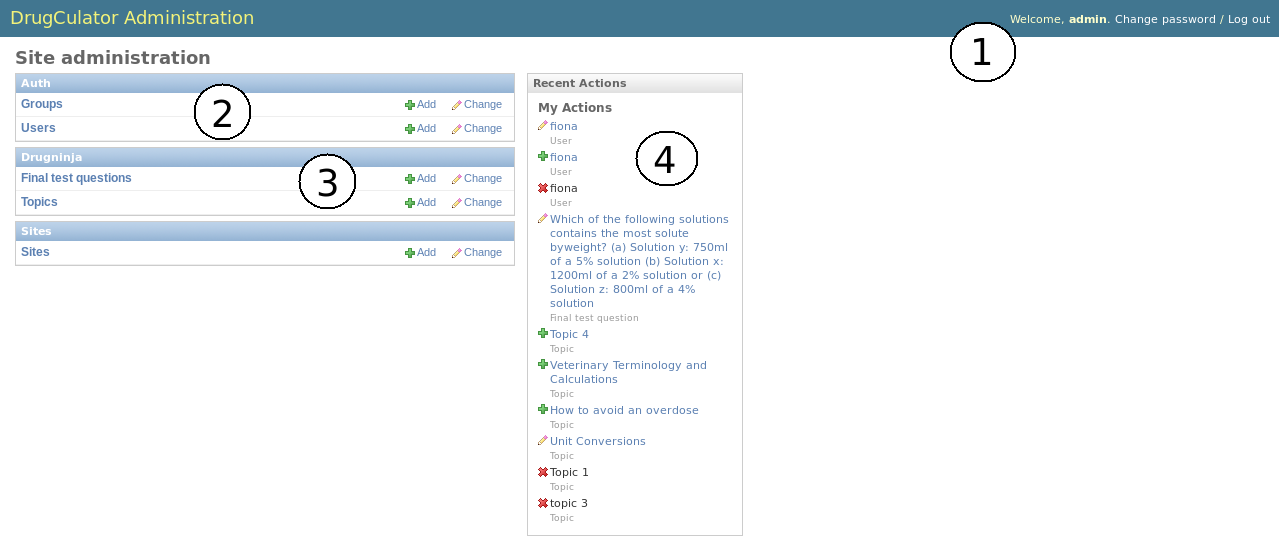
\includegraphics[width=\linewidth]{/users/level3/1002336a/TP3/team-project/Dissertation/images/admin_interface1.png}
\end{figure}

Figure (x.x) shows the main page of the admin interface after the admin user has logged in. The interface's specific design theme was largely out of our hands as Django provided this for us. The lack of design control wasn't an issue however, as it conformed to our earlier design goals that the interface should be sufficiently different in theme and style from the student user interface. As figure (x.x) shows, the overall theme is quite minimalistic. There is no extraneous details or features that could distract the admin user.

Annotation 1 shows the welcome message and menu for the user that has just logged into admin interface. It's placement at the top right hand side of the screen adheres to current best practise in web development, which in turn increases the usability of the interface. In terms of typography, the use of bold text confidently directs the user's eye towards expected features such as ``Change password'' and ``Log out''.

Annotation 2 highlights several of the user administration use cases in that they should be able to add, remove and edit current users within the application. These options are displayed logically by being grouped together and have icons that adhere to common user interface idioms. For example the ability to add a user is annotated with a plus symbol, enabling inexperienced users to intuitely deduce how that function would operate. 

Annotation 3 covers the content administrator's functional requirements in being able to add, edit and remove topic content. This annotation's style is identical to that of annotation 2, in that it contributes to the overall consistency of the admin user interface, providing a clear and usable experience for the user. As with annotation 2 a clearly recognisable icon (a pencil) is used to indicate that the link in question leads to editing options for the topics. 

Annotation 4 shows the ``Recent Actions'' bar of the interface. This enables admin users to see all their previous administrative actions for the application. This is very useful as it allows the administrator to track down previous changes to content and navigate to them directly. This navigation is further enhanced by the blue colour of the text, indicating that the text is a link and can be clicked. This blue text link consistency greatly adds to the expected functionality and to the usability of the interface as a whole.

The only design issue we faced with the admin user interface was the lack of creative control over the look and feel. While we still felt it was appropriate and suitably met our design considerations, it would have been better if Django allowed us greater customisation.

\subsection{Student User Interface}

\subsubsection{Main Content Screen}

\begin{figure}[!htb]
\caption{Content Screen}
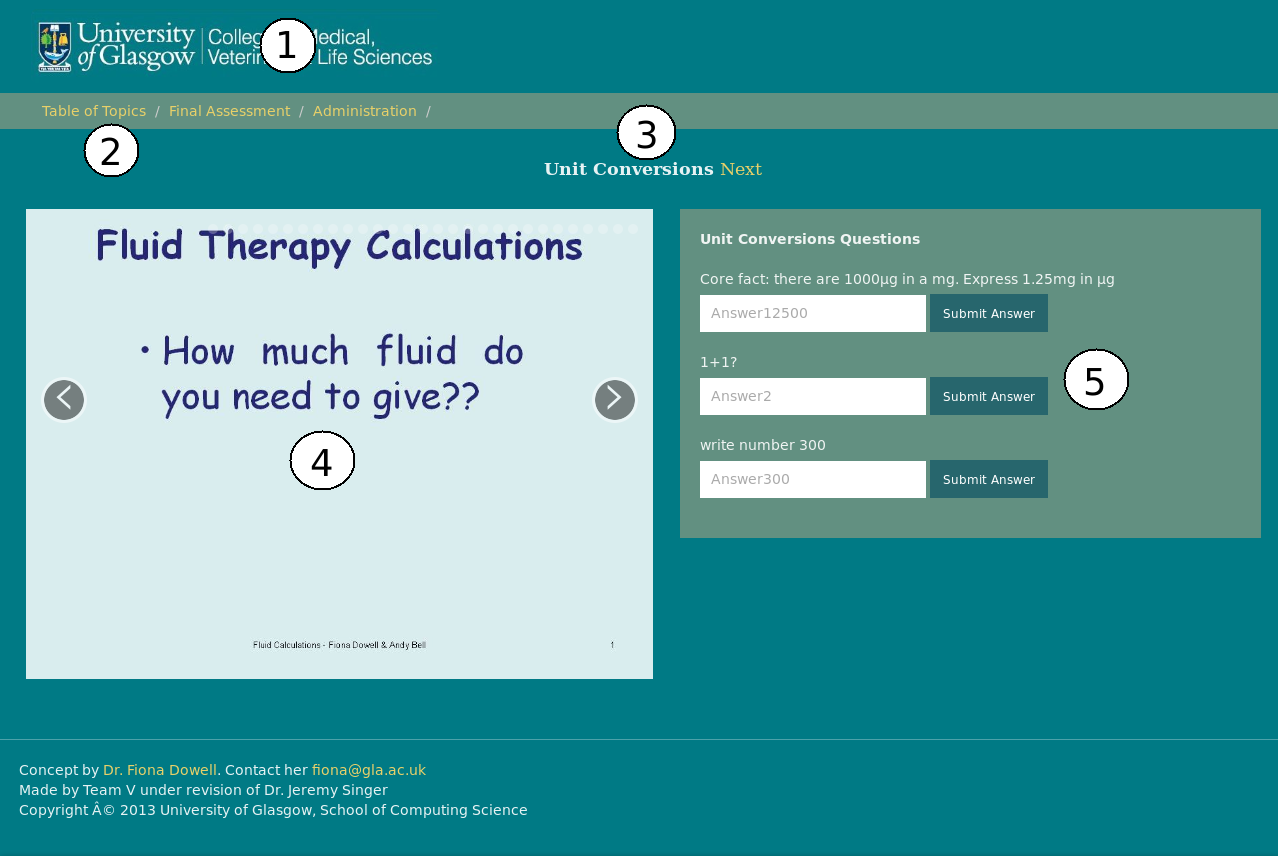
\includegraphics[width=\linewidth]{/users/level3/1002336a/TP3/team-project/Dissertation/images/topic_page_annotated.png}
\end{figure}

Figure x.4 shows the main page users will see when they interact with the system.

Annotation 1 highlights the image of the University of Glasgow's Veterinary School logo. This was included for two reasons: firstly it identifies the University to external bodies that may stumble across the application. Secondly it makes it appear more professional and therefore improves the overall aesthetics.

Annotation 2 shows the application's main navigation section. These are clearly labelled for clarity to identify their purpose. This also has the additional property of increasing usability. Expert users such as students who have used the program before and want to jump to a specific page can utilise these navigational tools quickly.

Annotation 3 is the sequential navigator for proceeding through topics. Depending on the topic selected there will also be a back button included. This function once again increases the usability of the application as well as adding to consistency to the design by providing a constant frame for content.

Annotation 4 is the final function available for navigation. This is our main content window where topic slides are displayed. When the mouse is hovered over the slide an arrow appears on either side of the screen to facilitate navigation. The use of arrows promotes recognition rather than recall for the user. 

Annotation 5 shows the questions associated with each topic. Each question is affiliated with a slide and users can answer them in their own time. This promotes the interactive learning element of the application. Each question gives instant feedback upon submission by altering the text in the box to display ''Correct Answer`` or ''Wrong Answer.`` 

\subsubsection{Final Assessment Screen}

\begin{figure}[!htb]
\caption{Final Assessment}
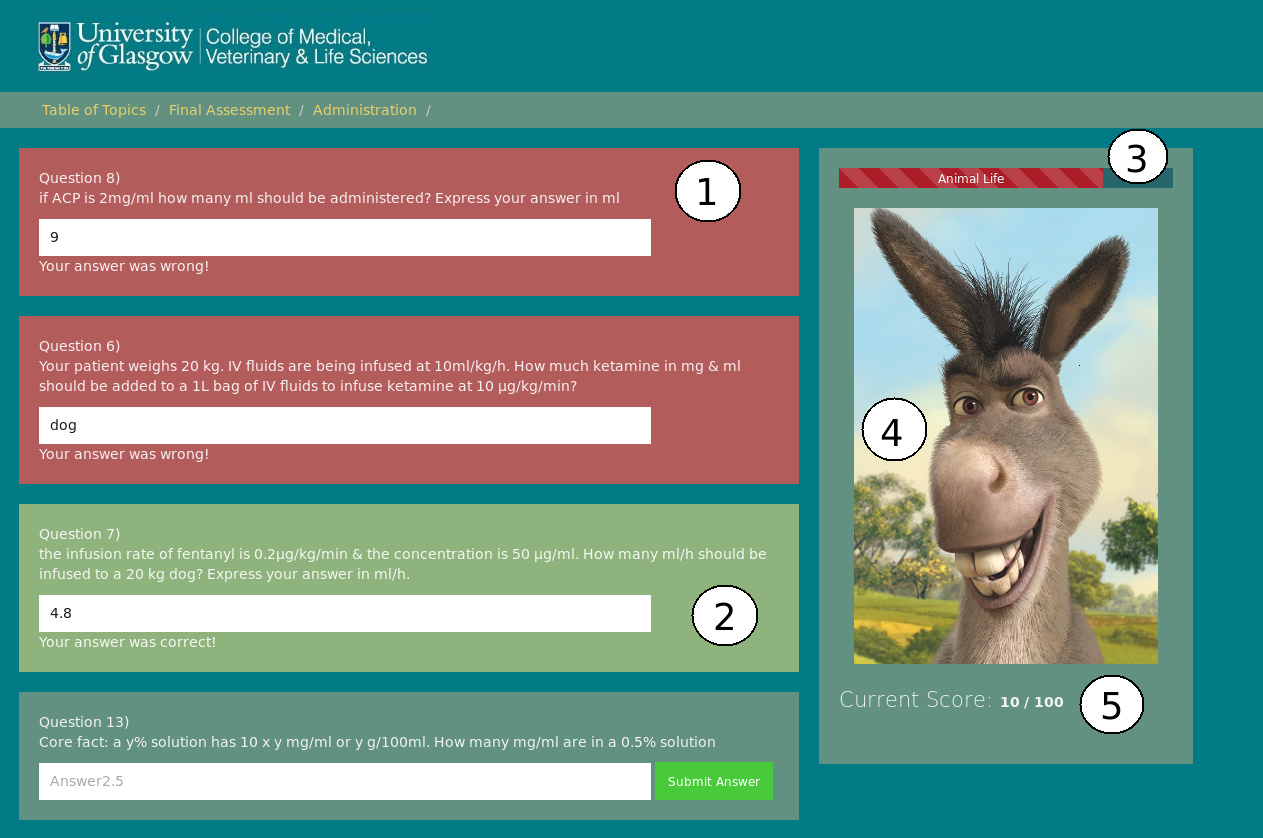
\includegraphics[width=\linewidth]{/users/level3/1002336a/TP3/team-project/Dissertation/images/annotated_assessment.png}
\end{figure}

Figure x.5 shows the assessment section of the application which presumably will be accessed when the user feels suitably prepared for it.

Annotation 1 shows an example of a question being answered wrong. Feedback is instantaneous with the question background changed to a subtle red colour, this is an intentional design decision to keep users engaged and willing to learn without discouraging them. Textual feedback is also provided for futher clarification. 

Annotation 2 shows an answer that is correct. This time the colour has changed to a slightly lighter green colour. Both the correct and incorrect colours are intrusive and fit with the design so as to keep the overall look pleasing.

The following three annotations illustrate the gamification of our application. By including the following elements we hope to engage users more effectively and provide an insentive to learn. Firstly they will attain a higher score and secondly they will keep the animal alive.

Annotation 3 is a progress bar which portrays the remaining health of the animal. For every wrong answer the bar will decrease indicating you hurt the animal (as a vet would do if they got these calculations wrong in the real world). Insentive to keep the animal alive will hopefully encourage the suer to get as many right answers as possible.

Annotation 4 is an image of the animal the students attempting to keep alive. For every decrement of 30 points the image changes to a steadily unhealthier looking donkey eventually resulting in a ``dead'' donkey. As with annotation 3 it is included to spur users to anser questions correctly.

Annotation 5 shows the users current score. This increases by ten points for every correct answer submitted and does not increase with wrong answers. 

\section{Conclusion}

The main focus of the design for the entirety of the application was to provide an interface that would be easy to use and reduce user frustration. Throughout development the idea of keeping users engaged with their learning and the content has been at the forefront and with the inclusion of a ``game'' of sorts on the final assessment the team believes they have succeeded in achieving this.




\end{document}
